\subsection{Versuchsaufbau}
Wie in Abb. 1 dargestellt ist das Americium-Präparat in einem evakuierten Glaszylinder befestigt, um den Druck zu verändern bzw. den Glaszylinder zu evakuieren, wird eine Vakuumpumpe benutzt. Der Halbleiter-Sperrschichtzähler dient, wie in der Theorie beschrieben als Detektor, danach wird der Impuls im Vorverstärker noch verstärkt, um dann mit dem Multichannel Analyzer (MCA) am Computer mithilfe einer Software die Daten auszuwerten. Das Präparat ist im Glaszylinder entlang einer Achse verschiebbar.

\subsection{Messung zur Reichweite der $\alpha$-Strahlung}

Zur Bestimmung der Reichweite der $\alpha$-Strahlung, wird bei
festgelegtem Abstand zwischen Strahlenquelle und Detektor die Anzahl der Stromimpulse bei verschiedenen Drücken gemessen. Es wird pro Druck \SI{120}{\second} lang gemessen. Dabei wird mit einem
Druck von annähernd \SI{0}{\milli\bar} begonnen, anschließend wird der Druck bis \SI{400}{\milli\bar} um \SI{100}{\milli\bar} pro Messung erhöht, danach in \SI{50}{\milli\bar} Schritten bis Normaldruck erreicht ist. Die Messung wird für einen leicht veränderten Abstand noch einmal wiederholt.\\

Die effektive Länge $x$ lässt sich bei festem Abstand $x_0$ zwischen
Strahlenquelle und Detektor in Abhängigkeit vom Druck $p$ im Glaszylinder angeben.

\begin{equation}
  \label{eq:effektive_laenge}
  x = x_0 \cdot \frac{p}{p_0}
\end{equation}

Die effektive Länge gibt an, wie groß der Abstand zwischen Strahlenquelle und Detektor sein müsste, wenn die Messung bei festem Atmosphärendruck $p_0$ durchgeführt würde, um ein äquivalentes Verhalten der Anzahl der ankommenden $\alpha$-Teilchen zu erhalten in Relation zum eingestellten Druck $p$. Dadurch kann man die Reichweite der Teilchen durch Variation des Druckes bestimmen.
 
\subsection{Messung zur Statistik des radioaktiven Zerfalls}
Im letzten Versuchsteil werden für einen festen Abstand (Präparat/Detektor) im evakuierten Glaszylinder alle \SI{10}{\second} die Zerfälle gemessen. Dies wird 100 mal wiederholt, damit eine statistische Aussage getroffen werden kann.

\begin{figure}[h]
  \centering
  \label{fig:Versuchsaufbau}
  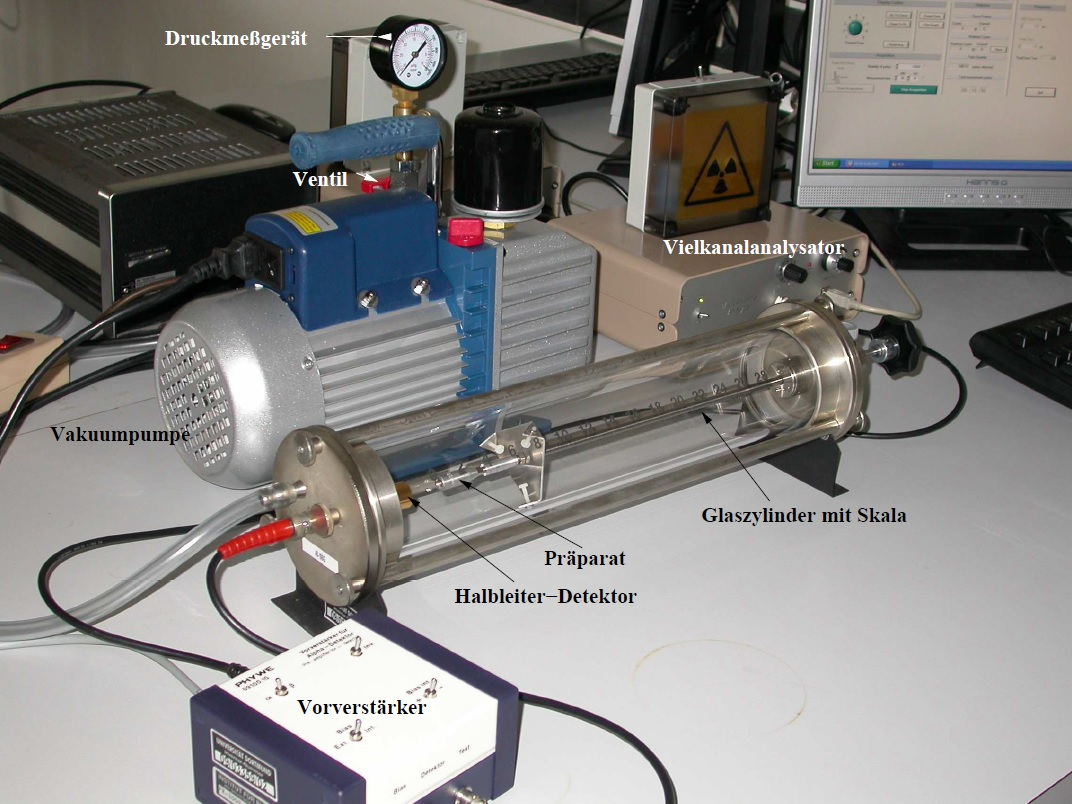
\includegraphics[width=0.9\textwidth]{Grafiken/V701_Versuchsaufbau.jpg}
  \caption{Versuchsaufbau zur Messung der Reichweite von $\alpha$-Strahlung}
\end{figure}
